% INTRODUÇÃO-------------------------------------------------------------------

\chapter{INTRODUÇÃO}
\label{chap:introducao}

Os avanços tecnológicos da humanidade cresceu na últimas décadas. 
Consequentemente houve um aumento na exploração dos recursos marinhos, fazendo dos oceanos uma fonte para a satisfação de diversas demandas humanas.
Além disso, houve um crescente desenvolvimento de ferramentas robóticas para exploração e atuação nestes ambientes.
Apesar dos avanços proporcionados pela robótica subaquática, ainda há muitos desafios para enfrentar. 
Entre as dificuldades no desenvolvimento da área, estão: turbidez da água, que impede a visualização com sensores ópticos; pressão, dependendo da profundidade pode dificultar na logística e no acesso humano; equipamentos, dispositivos e tecnologias com alto custo de aquisição; entre outros. 

Uma alternativa para contornar alguns dos problemas e avançar nas pesquisas é usufruir dos avanços da tecnologia computacional e utilizar a simulação virtual.
As simulações proporcionam dados próximos aos dados adquiridos em um experimento real, além de requerer baixo custo (financeiro e de tempo) comparados à um experimento em campo. 
Outra alternativa é estudar maneiras de adquirir um melhor aproveitamento de sensores menos robustos e mais acessível.
A utilização de sensores com baixo custo financeiro aliado à simulações virtuais é um caminho para realizar grandes avanços na área com poucos recursos.

\section{Motivação}
\label{sec:motivacao}

O aquecimento global é o processo de aumento da temperatura média da superfície terrestre e dos oceanos, causado por uma grande quantidade de gases, como o dióxido de carbono ($CO_2$) e o metano ($CH_4$), originados de atividades humanas e emitidos na atmosfera terrestre provocando grandes impactos ambientais negativos. Os principais impactos causados pelo aquecimento global são: aumento de eventos de extremo climático (ciclones, ondas de calor, chuvas torrenciais, etc), redução de biodiversidade, elevação do nível do mar e da temperatura na superfície terrestre, etc. 

A temperatura da superfície global aumentou cerca de 0.2 \textordmasculine C em três décadas e 0.8 \textordmasculine C no último século \cite{hansen2006global}. Para ilustrar esse retrato, a Figura \ref{fig:ast-and-sl}-A mostra as mudanças na temperatura média da superfície terrestre enquanto a Figura \ref{fig:ast-and-sl}-B exibe as mudanças no nível médio do mar. Essas mudanças ocorreram no intervalo de 1986 a 2005.

\begin{figure}[H]
    \centering
    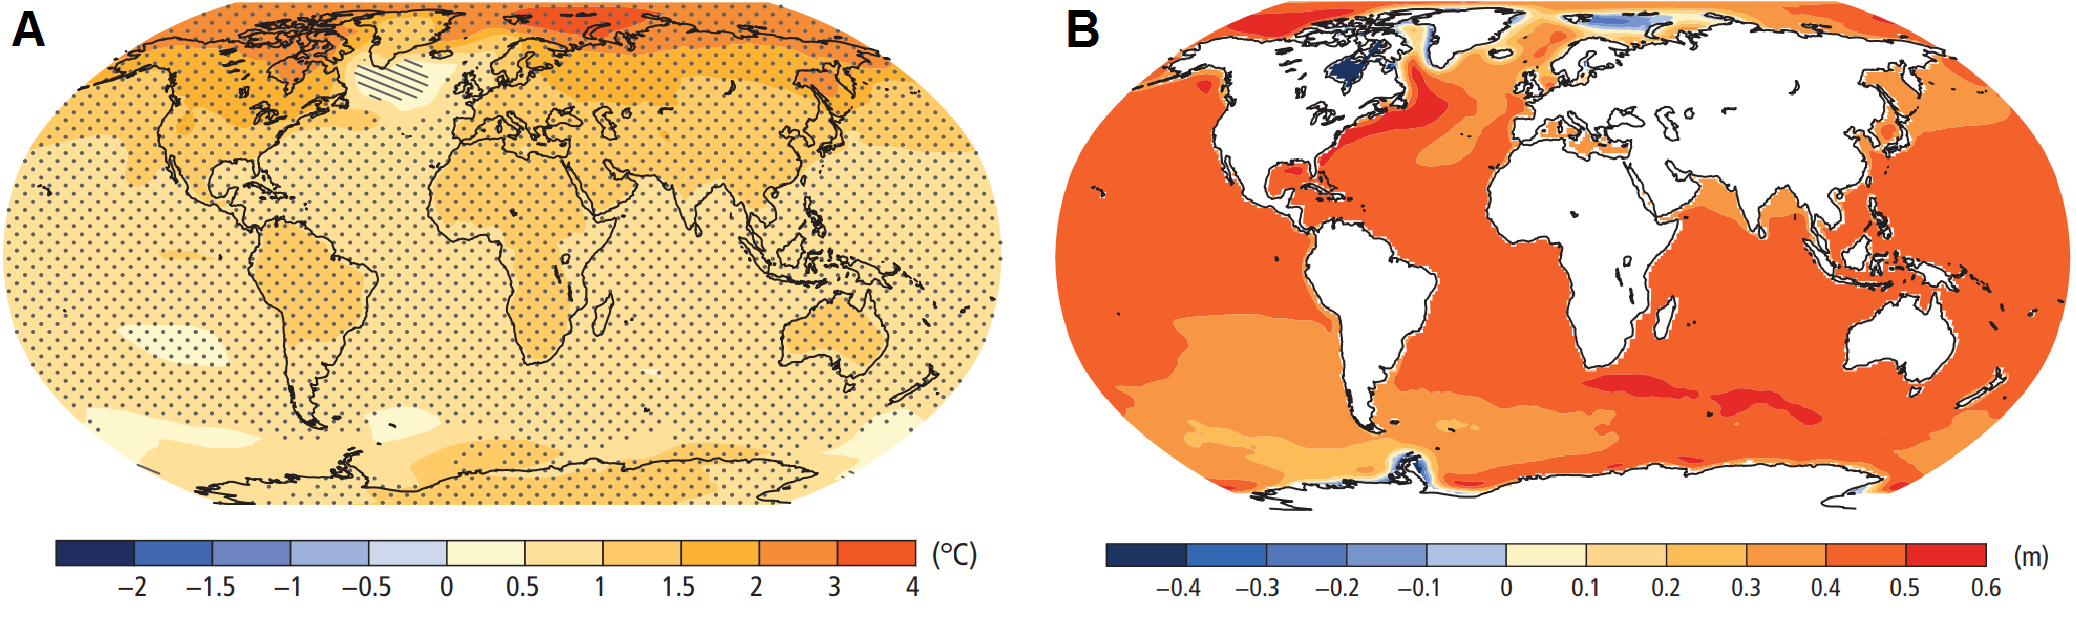
\includegraphics[scale=0.27]{dados/figuras/ast-and-sl.png}
    \caption{(A) Mudança na temperatura média da superfície terrestre (1986 -- 2005). (B) Mudança do nível médio do mar (1986 -- 2005).}
    \vspace{-0.8em}
    \fonte{Adaptado de \cite{pachauri2014climate}.}
    \label{fig:ast-and-sl}
\end{figure}

A redução da criosfera é um dos problemas ocasionado pelo aumento da temperatura e do nível do mar. A criosfera é constituída por regiões da superfície terrestre cobertas permanentemente por gelo e neve ou o solo é constituído por gelo, como por exemplo: lagos e rios congelados, mantos e calotas de gelo, neve sazonal e geleiras.

Em destaque, as geleiras do planeta estão perdendo massa, tornando uma das principais causas para o aumento no nível dos oceanos \cite{rietbroek2016revisiting}. Devido a importância econômica, ao seu papel como indicador de mudança no clima, além de ser o maior reservatório de água doce sobre a Terra, perdendo em volume total de água apenas para os oceanos \cite{pinto2015crise}, o monitoramento das geleiras se torna indispensável para o planeta.

Entretanto, a maior parte das geleiras estão em locais remotos, dificultando o acesso e a logística à essas áreas. 
Por consequência, os estudos com o sensoriamento remoto se tornou uma alternativa comumente utilizada para a estimação de balanço de massa, como mostra os trabalhos de \cite{rojas2016darwin} e de \cite{mendonca2013greyglacier}.
Porém, os satélites não são eficazes para coletar informações de geleiras que possuem uma parcela submersa, visto que a tecnologia do sensoriamento remoto só captura informações da superfície terrestre, impedindo coletar informações a respeito do que está entre a superfície e o fundo de corpos d'água. 
A Figura \ref{fig:remote_sensor} mostra o mecanismo de aquisição de dados do sensoriamento remoto. A obtenção de informações é realizada por meio do registro do retorno da interação da radiação eletromagnética provida do Sol com a superfície terrestre. 

\begin{figure}[H]
    \centering
    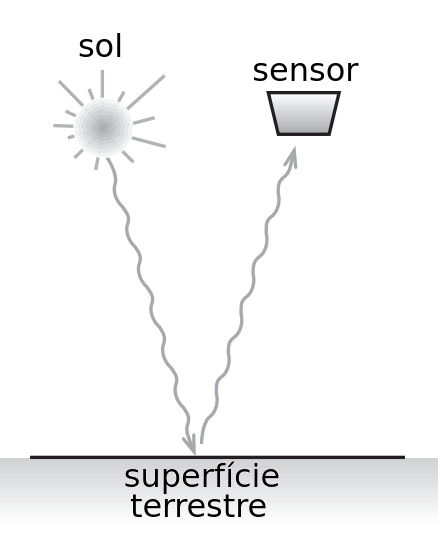
\includegraphics[scale=0.5]{dados/figuras/remote_sensor.png}
    \caption{Aquisição de dados do sensoriamento remoto.}
    \vspace{-0.8em}
    \fonte{Adaptado de \cite{kerle2004principles}.}
    \label{fig:remote_sensor}
\end{figure}

Para coletar informações em ambientes submersos torna-se mais adequado utilizar sensores que operam com ondas sonoras, pois essas se propagam melhor em ambientes com maior densidade, como o fundo de oceanos e lagos.

\section{Desafios}
\label{sec:desafios}

A coleta submersa só é possível com o auxílio de um robô submarino operado de forma remota, sendo necessário superar alguns desafios.
Um deles é usar dispositivos com baixo custo, pois o risco de perda do equipamento e o custo são altos, visto que grande parte dos ambientes submersos são profundos e possui baixas temperaturas.
Além disso, outros problemas do ambiente influenciam na aquisição dos dados, como a correnteza que impede o ROV de se manter inerte e a turbidez da água que atrapalha a visualização do robô pelo operador.

Na etapa de manipulação dos dados, o desafio está em utilizar métodos eficazes para remover o máximo de ruído e perdendo o mínimo de informações.
Do mesmo modo, o desafio da reconstrução será encontrar uma metodologia capaz de fazer a reconstrução alcançar o mais próximo do real.


\section{Objetivos}
\label{sec:objetivos}

O objetivo principal do trabalho é utilizar uma plataforma robótica do tipo ROV (Robô Operado Remotamente, do inglês \textit{Remotely Operated Vehicle}) equipada com um sensor sonar MSIS (do inglês \textit{Mechanical Scanning Image Sonar}) para estimar variações espaciais (balanço de massa) de superfícies submersas por meio da reconstrução em 3D de capturas temporalmente espaçadas de imagens acústicas. 
Para atingir o objetivo principal, será necessário alcançar tais objetivos específicos:

\begin{itemize}
    \item Estudar o mecanismo e eficiência da aquisição de imagens do sonar MSIS e os principais métodos para manipular imagens acústicas;
    \item Coletar dados em simulação e \textit{in loco} utilizando robô subaquático acoplado com sonar e sensores auxiliares;
    \item Reconstruir as superfícies submersas utilizando algoritmos de reconstrução com o auxílio de bibliotecas de nuvem de pontos e de geometria;
    \item Simular o ambiente para avaliar a metodologia proposta;
    \item Comparar modelos reconstruídos com o intuito de analisar a perda/ganho de volume entre eles.
\end{itemize}
\hspace{1em}

Para a efetivação dos objetivos, o NAUTEC (Grupo de Pesquisa em Automação e Robótica Inteligente) junto ao C3 (Centro de Ciências Computacionais), disponibilizará a plataforma robótica, o sensor sonar e sensores auxiliares. Este trabalho é o inicio dos estudos para uma melhor precisão na estimação da ablação\footnote{Ablação é a perda de massa/energia de um sistema, nessa circunstância, a fusão e sublimação do gelo.} e o conhecimento de características da parte frontal submersa de geleiras, tais como configuração física e comportamento de degelo, que será uma contribuição com o LACRIO (Laboratório de Monitoramento da Criosfera). Além disso, o trabalho contribuirá para a consolidação da área da robótica subaquática na FURG (Universidade Federal do Rio Grande).
Embora o trabalho prático seja realizada em ambiente não glacial, a intenção é dar continuidade ao projeto e, posteriormente ser executado em geleiras.


\section{Organização do trabalho}
\label{sec:organizacaoTrabalho}

A organização do trabalho está separada em 5 capítulos, nos quais estão configurados na seguinte forma.
Após o capítulo de introdução, o Capítulo \ref{chap:fundamentacaoTeorica} apresenta assuntos fundamentais para a compreensão do mesmo, como a descrição do sensor e dos \textit{softwares} utilizados. No Capítulo \ref{chap:metodologia}, é abordado detalhadamente a metodologia utilizada e seus motivos. O Capítulo \ref{chap:resultados} apresenta os resultados que foram obtidos no experimento real e em simulação. 
Por último, o Capítulo \ref{chap:conclusao} encerra o trabalho com a conclusão do autor sobre o desenvolvimento e resultados obtidos.